\section{Erhalt erster Integrale}

Betrachte die autonome Differentialgleichung
\begin{equation*}
	x'=f(x)
\end{equation*}
auf einem Phasenraum $\Omega_0$.

\begin{definition}
 Eine Funktion $\mathcal E:\Omega_0\to\R$ heißt \emph{erstes Integral}, wenn
 \begin{equation*}
		\mathcal E(\Phi^t x) = \mathcal E(x)
	\end{equation*}
 für alle $x\in\Omega_0$ und alle zulässigen $t$ gilt.
\end{definition}

	Alternative Bezeichnungen:
	\begin{itemize}
		\item Invariante
		\item Erhaltungsgröße
 \item engl.: constant of motion
	\end{itemize}

\emph{Beispiel:} Mathematisches (Faden-)pendel\\
\begin{figure}[h]
\begin{center}
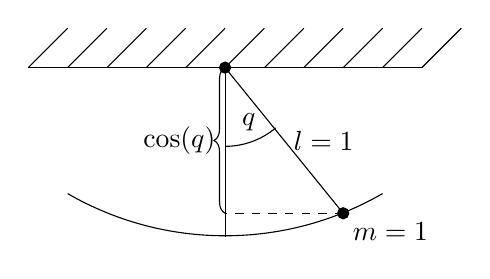
\begin{tikzpicture}
\draw (0,4) -- (5,4);
\foreach \i in {0,...,10}
\draw (\i / 2, 4) -- ( \i/2+ 0.5, 4.5);
\draw[fill] (2.5,4) circle (2pt);
\draw[fill] (4,2.15) circle (2pt) node[below right]{$m=1$};
\draw (0.5,2.4) arc (-120:-60:4);
\draw  (2.5,4) -- node[right]{$l=1$} (4,2.15) ;
\draw (2.5,4) -- (2.5,1.85);
\draw[dashed] (4,2.15) -- (2.5,2.15);
\draw (2.5, 3) arc (-90:-50:1);
\draw (2.8,3.3) node {$q$};
\draw [decorate,decoration={brace,amplitude=4pt}]
(2.5,2.15)--(2.5,4) node[midway, left] {$\cos(q)$};
\end{tikzpicture}
\end{center}
\end{figure}

Bewegungsgleichungen für Winkel $q$:
\begin{align*}
 \ddot{q} + \frac{g}{l} \sin q = 0
\end{align*}
bzw.\ als System erster Ordnung:
\begin{align*}
\dot{p} &= - mgl \sin q\\
\dot{q} &= \frac{1}{ml^2} p.
\end{align*}
Erhält $\mathcal E(p,q) = \frac{1}{2} \frac{1}{ml^2} p^2 - mgl \cos q $ (die totale Energie).\\

\emph{Beispiel:} Betrachte ein System mit $N$ Partikeln
\begin{itemize}
	\item $q_i\in\R^3,\ i=1,\hdots,N$ Positionen, $p_i\in\R,\ i=1,\hdots,N$ Impulse
        \item $m_i$: Massen
 \item Paarweise Interaktion über Kräfte, die vom Abstand abhängen.
\end{itemize}
Bewegungsgleichungen:
\begin{equation*}
	q_i'=\frac{p_i}{m_i},\qquad p_i' = \sum_{j=1}^N \nu_{ij}(q_i-q_j)
\end{equation*}
mit
\begin{align*}
 \nu_{ij}(y) = - \nu_{ji}(-y)
\end{align*}
daraus folgt insbesondere dass $\nu_{ii} = 0$.

Die Bewegungsgleichungen erhalten den Gesamtimpuls $P=\sum_{i=1}^Np_i$, denn
\begin{equation*}
 \frac{d}{dt}\sum_{i=1}^Np_i = \sum_{i=1}^N p_i' = \sum_{i=1}^N\sum_{j=1}^N\nu_{ij}(q_i-q_j) = 0
\end{equation*}
Ebenso: Der Gesamtdrehimpuls $L=\sum_{i=1}^N q_i\times p_i$
\begin{align*}
\frac{d}{dt}\sum_{i=1}^N q_i\times p_i
 & = \sum_{i=1}^N q_i'\times p_i+\sum_{i=1}^N q_i\times p_i' \\
 %
 & = \sum_{i=1}^N \frac{1}{m_i}\underbrace{p_i\times p_i}_{=0} + \sum_{i=1}^N\sum_{j=1}^Nq_i\times\nu_{ij}(q_i-q_j) \\
 %
 & = 0.
\end{align*}
Klassifikation der Erhaltungsgrößen: (für diese Beispiele)
\begin{itemize}
 \item Impuls: linear
 \item Drehimpuls: quadratisch
 \item Energie beim Fadenpendel: nichtlinear
\end{itemize}
Man hätte gerne numerische Verfahren, die erste Integrale erhalten.

\medskip

Zunächst eine einfache Charakterisierung mit Hilfe von $f$:
\begin{lemma}[{{\cite{deuflhard_bornemann:2008}}} 6.56]
 Sei $f$ lokal Lipschitz-stetig. Eine Funktion $\mathcal E\in C^1(\Omega_0,\R)$ ist genau dann
 erstes Integral, wenn
 \begin{equation*}
  \nabla\mathcal E(x)\cdot f(x) = 0
	\end{equation*}
	für alle $x\in\Omega_0$.
\end{lemma}
\begin{proof}
	Kettenregel:
 \begin{equation*}
  0
  =
  \frac{d}{dt} \mathcal E(\Phi^t x)
  =
  \nabla\mathcal E(\Phi^tx)\cdot \frac{d}{dt}\Phi^tx
  =
  \nabla\mathcal E(\Phi^tx)\cdot f(\Phi^tx).  
\end{equation*}
\end{proof}

\bigskip

\emph{Beispiel:} Wir zeigen Energieerhaltung des Fadenpendels.
Für dieses Modell gilt:
\begin{align*}
 f(x) & = f(p,q)
  =
  \begin{pmatrix}
   - mgl \sin q \\ \frac{p}{ml^2}
  \end{pmatrix} \\
 %
 \mathcal{E}(x) & = \mathcal{E}(p,q)
  =
  \frac{1}{2} \frac{p^2}{ml^2} - mgl \cos q
\end{align*}
Der Gradient der Energie ist
\begin{equation*}
 \nabla \mathcal{E}(p,q)
 =
 \begin{pmatrix}
  \frac{p}{ml^2} \\ mgl \sin q
 \end{pmatrix}
\end{equation*}
Damit erhält man
\begin{equation*}
 \nabla \mathcal{E}(p,q) \cdot f(p,q)
 =
 \frac{p}{ml^2}(- mgl \sin q) + mgl \sin q\frac{p}{ml^2}
 =
 0.
\end{equation*}



\bigskip

\begin{satz}[{{\cite[Thm.\ IV.1.5]{hairer_lubich_wanner:2006}}}]
	Alle Runge-Kutta-Verfahren erhalten lineare Invarianten.
\end{satz}
\begin{proof}\mbox{}
	\begin{itemize}
		\item Sei $\mathcal{E}$ lineare Invariante, also $\mathcal{E}(x) = d^Tx$ mit festem Vektor $d$.
		\item Nach dem vorigen Satz ist dann $d^T f(x) = 0$ für alle $x\in\Omega_0$.
		\item Für eine Stufe $k_i$ eines beliebigen RK-Verfahrens ist dann
		\begin{equation*}
			d^T k_i = d^T f\Big( x+\tau\sum_{j=1}^s a_{ij}k_j \Big) = 0.
		\end{equation*}
		\item Also ist
		\begin{equation*}
			\mathcal E(x_{k+1})
			=
			d^T x_{k+1}
			=
			d^T\Big(x_k+\tau\sum_{i=1}^s b_{i}k_i\Big)
			=
			d^T x_k
			=
			\mathcal{E}(x_k).   
		\end{equation*}
		\end{itemize}
\end{proof}

Für die quadratischen Invarianten betrachten wir zunächst einen wichtigen Spezialfall:

\medskip

\emph{Frage:} Für welche linearen autonomen Differentialgleichungen
\begin{equation*}
 x'=Ax
\end{equation*}
erhält der Phasenfluss $\Phi^t$ die Euklidische Norm
\begin{equation*}
	\norm{\Phi^t x}_2 = \norm{x}_2\quad\forall t?
\end{equation*}
$\Rightarrow$ Genau dann, wenn $\Phi^t = \exp(tA)$ eine orthogonale Matrix ist.
\begin{satz}[{{\cite[6.18]{deuflhard_bornemann:2008}}}]
\label{thm:normerhaltende_fluesse}
 Sei $A\in\R^{d \times d}$. Die Matrix $\exp(tA)$ ist genau dann orthogonal,
 wenn $A$ schiefsymmetrisch ist.
\end{satz}
\begin{proof}
 Teil~I) $\exp(tA)\in O(d) \Rightarrow A=-A^T$
 \begin{itemize}
  \item Sei $\exp(tA)\in O(d)$ für alle $t$.
  \item Dann ist
   \begin{equation*}
    I = \exp(tA)^T \exp(tA) = \exp(tA^T) \exp(tA).
   \end{equation*}
 \item Differenziere nach $t$ und betrachte $t=0$
  \begin{equation*}
   0=\Big(A^T \exp(tA^T) \exp(tA) + \exp(tA^T)A \exp(tA) \Big)\Big|_{t=0} = A^T+A
  \end{equation*}
	\end{itemize}
 Teil~II) $A=-A^T \Rightarrow \exp(tA)\in O(d)$
 \begin{align*}
	 I
	 &= \exp(tA-tA) = \exp(tA)\cdot \exp(-tA)\quad\text{(da $A$ mit $A$ kommutiert)}\\
	 &= \exp(tA)\cdot \exp(tA^T) \\
	 &= \exp(tA)\cdot \exp(tA)^T	 
 \end{align*}
\end{proof}
Zentral ist anscheinend die Eigenschaft
\begin{equation*}
	\exp(z)\cdot \exp(-z) = 1\qquad \forall z\in\C.
\end{equation*}
Das nennt man \emph{Reversibilität}.

\medskip

Man hätte diese Eigenschaft gerne auch für diskrete Verfahren.
\begin{definition}
	Eine diskrete Evolution $\Psi$ heißt reversibel, wenn
	\begin{equation*}
		\Psi^{t,t+\tau}\Psi^{t+\tau,t} x = x
	\end{equation*}
	für alle $(t,x)\in\Omega$ und hinreichend kleine $\tau$.
\end{definition}

\emph{Beispiel:} Das explizite Euler-Verfahren ist nicht reversibel.

\medskip

Reversible rationale Approximationen der Exponentialfunktion erzeugen normerhaltende diskrete Flüsse.

\begin{satz}[Db\,\&\,Bo 6.21]
	Sei $R$ eine rationale, konsistente, reversible Approximation der Exponentialfunktion. Dann gilt für eine Matrix $A\in\R^{d\times d}$
	\begin{equation*}
		R(\tau A)\in O(d)\qquad\forall \tau > 0
	\end{equation*}
	genau dann, wenn $A=-A^T$.
\end{satz}
\begin{proof}
 Weitestgehend wie bei Satz~\ref{thm:normerhaltende_fluesse}.
\end{proof}
\emph{Beispiel:}
\begin{equation*}
	R(z) = \frac{1+\frac{z}{2}}{1-\frac{z}{2}}=1+z+\frac{z^2}{2} + \frac{z^3}{4} + \mathcal{O}(z^4) = e^z + \mathcal O(z^3)
\end{equation*}
\begin{itemize}
	\item Die entsprechende Matrix-Abbildung heißt \emph{Cayley-Transformation}.
	\item Stabilitätsfunktion insbesondere der impliziten Mittelpunktsregel\\
	$\rightarrow$ dem einfachsten Gauß-Verfahren.
\end{itemize}
Gauß-Verfahren erhalten sogar beliebige quadratische Invarianten!
\begin{satz}[{{\cite[6.58]{deuflhard_bornemann:2008}}}]
	Die D.Gl. $x'=f(x)$ mit lokal Lipschitz-stetigem $f$ besitze das quadratische erste Integral $\mathcal E$, d.h.
	\begin{equation*}
		\mathcal E(x) = x^TEx + e^Tx + \eta
	\end{equation*}
	mit $E\in\R^{d\times d},\ e\in\R^d,\ \eta\in\R$. Jedes Gaus-Verfahren erzeugt einen Phasenfluss $\Psi$, der $\mathcal E$ erhält, d.h.
	\begin{equation*}
		\mathcal E(\Psi^\tau x) = \mathcal E(x)
	\end{equation*}
	für alle $x\in\Omega_0$ und  zulässige $\tau$.
\end{satz}
\begin{proof}
	Ganz ähnlich wie der Beweis der $B$-Stabilität.
	\begin{itemize}
		\item  Sei $x\in\Omega_0$, und $\tau$ so klein, dass das Kollokationspolynom
		\begin{equation*}
			u\in P_s,\quad u(0)=x,\quad u(\tau) = \Psi^\tau x
		\end{equation*}
		existiert.
		\item $\mathcal E$ ist quadratisch. Deshalb ist
		\begin{equation*}
			q(\theta) \colonequals \mathcal E(u(\theta\tau))
		\end{equation*}
		ein Polynom in $P_{2s}$.
		\item Hauptsatz der Integralrechnung:
		\begin{equation*}
			\mathcal E(\Psi^\tau x) = q(1) = q(0) + \int_0^1q'(\theta)\,d\theta = \mathcal E(x) + \int_0^1q'(\theta)\,d\theta . 
		\end{equation*}
		\item Zu zeigen ist also $\int_0^1q'(\theta)\,d\theta =0$.
		\item Nutze Quadraturformel des Gauß-Verfahrens.\\
		Diese ist für Polynome in $P_{2s-1}$ exakt:
		\begin{equation*}
			\int_0^1q'(\theta)\,d\theta = \sum_{j=1}^s b_j q'(c_j).
		\end{equation*}
		\item Es sind aber alle $q'(c_j)=0$, denn
		\begin{align*}
		q'(c_j) &= \big(\mathcal E(u(c_j\tau))\big)'\\
		   &= \tau\nabla\mathcal E(u(c_j\tau))\cdot u'(c_j\tau)\quad\text{(Kettenregel)} \\
		   &= \tau\nabla\mathcal E(u(c_j\tau))\cdot f(u(c_j\tau))\quad\text{(Kollokationseigenschaft)}\\
		   &= 0\quad\text{(da $\mathcal E$ eine Invariante ist)}.
		\end{align*}
	\end{itemize}
\end{proof}
Was ist mit der Energieerhaltung des Fadenpendels?
\begin{itemize}
	\item Das behandeln wir später.
	\item Mit der Theorie der Hamiltonschen Systeme.
\end{itemize}